\section{Descrizione dell'architettura}
\subsection{Architettura frontend}
\subsubsection{Elenco dei componenti}
Poiché il team di sviluppo frontend utilizzerà Redux per la gestione dello stato, l'applicazione sarà strutturata principalmente attraverso la suddivisione del codice in slices, stati iniziali e azioni.
\paragraph{Slices}
    Le Slice contengono una porzione dello stato globale dell’applicazione che è gestita da un reducer
    specifico.
\begin{itemize}
        \item \textbf{DataSlice:} componente che gestisce lo stato e contiene i dati relativi al dataset selezionato dall'utente;
        \item \textbf{AppStateSlice:} componente che gestisce lo stato dell'applicazione come errori e caricamenti;
        \item \textbf{DataSourceSlice:} componente che gestisce lo stato e contiene l'elenco dei dataset selezionabili dall'utente e il dataset selezionato;
        \item \textbf{FilterOptionSlice:} componente che gestisce lo stato e contiene le opzioni di filtraggio, come la selezione di valori maggiori o minori.;
        \item \textbf{RaycastHitSlice:} componente che gestisce lo stato e contiene le informazioni relative al raycasting.
\end{itemize}
\paragraph{Initial states}
    Gli stati iniziali, definiti all'interno di ciascuna slice, si combinano per formare lo stato globale dell'applicazione, gestito dallo store.
    \begin{itemize}
        \item \textbf{RawDataInitialState:} componente che contiene i dati relativi al dateset selezionato dall'utente;
        \item \textbf{AppInitialState:} componente che contiene i dati relativi allo stato attuale dell'applicazione;
        \item \textbf{DataSoruceInitialState:} componente che contiene le informazioni principali di tutti i dataset e quelle relative al dataset selezionato dall'utente;
        \item \textbf{FilterOptionInitialState:} componente che contiene i dati relativi alle opzioni di filtraggio selezionate dall'utente;
        \item \textbf{RaycastHitInitialState:} componente che contiene i dati relativi al raycasting, utilizzati per l'interazione con le barre del grafico tridimensionale.
    \end{itemize}
\paragraph{Actions}
    LLe azioni, emesse dai componenti, vengono inviate ai reducers per aggiornare lo stato corrispondente.
    Ogni azione è caratterizzata da un type e da un payload, che viene utilizzato dalle slices per modificare lo stato.
    Per convenzione il nome delle azioni segue il formato: \\
    \begin{center}
        \textbf{[nome Slice dalla quale viene catturata].[nome azione]}.
    \end{center}
    \begin{itemize}
        \item \textbf{DataSlice.requestData:} azione asincrona emessa per recuperare, dal server, i dati del dataset selezionato; \\ Payload: nessuno
        \item \textbf{DataSlice.filterTopN:} azione emessa per filtrare i dati, visualizzando esclusivamente i top o bottom N valori; \\ Payload: FilterPayload
        \item \textbf{DataSlice.filterAboveValue:} azione emessa per filtrare i dati, visualizzando esclusivamente quelli con un valore maggiore o minore rispetto al valore selezionato;\\ Payload: FilterPayload
        \item \textbf{DataSlice.filterAverage:} azione emessa per filtrare i dati, visualizzando esclusivamente quelli con un valore maggiore o minore rispetto alla media globale; \\ Payload: boolean $\rightarrow$ maggiore o minore
        \item \textbf{AppStateSlice.setLoading:} azione emessa per aggiornare lo stato dell'applicazione e visualizzare la pagina di caricamento; \\ Payload: boolean
        \item \textbf{AppStateSlice.setError:} azione emessa per aggiornare lo stato dell'applicazione e visualizzare una schermata di errore specifica, basata sull'errore generato dall'applicazione; \\ Payload: number $\rightarrow$ codice di errore.
        \item \textbf{DataSourceSlice.requestDatasets:} azione asincrona emessa per recuperare l'elenco delle informazioni relative a tutti i dataset disponibili; \\ Payload: nessuno.
        \item \textbf{DataSourceSlice.setCurrentDataset:} azione emessa per aggiornare il dataset selezionato dall'utente; \\ Payload: string DatasetInfo.
        \item \textbf{FilterOptionSlice.toggleAveragePlane:} azione emessa per aggiornare il flag di visibilità del piano medio globale nell'ambiente tridimensionale; \\ Payload: boolean 
        \item \textbf{FilterOptionSlice.toggleIsGreater:} azione emessa per aggiornare il flag che determina se il filtraggio deve essere eseguito per valori maggiori o minori; \\ Payload: boolean
        \item \textbf{RaycastHitSlice.setHit:} azione emessa per aggiornare la barra selezionata nel grafico tridimensionale; \\ Payload: number $\rightarrow$ ID della barra.
        \item \textbf{RaycastHitSlice.setTooltipPosition:} azione emessa per aggiornare la posizione del tooltip in base alla posizione del puntatore.\\ Payload: Vector3 $\rightarrow$ posizione del puntatore.
    \end{itemize}
\paragraph{Classes}
    Classi offerte dalle librerie utilizzate:
    \begin{itemize}
        \item \textbf{Vector3:} classe offerta dalla libreria three.js. Rappresenta un vettore tridimensionale, ovvero
        una grandezza fisica caratterizzata da una direzione e da una lunghezza. Il vettore tridimensionale
        viene comunemente utilizzato per definire la posizione, la rotazione, la scala e la direzione
        delle barre del grafico tridimensionale;
        \item \textbf{Provider:} Componente Redux che rende lo store accessibile a tutti i componenti dell'applicazione, "avvolgendo" il componente principale App e accettando lo store come prop;
        \item \textbf{Store:} Lo store Redux traccia lo stato dell'applicazione, contiene il reducer principale per la gestione delle azioni e fornisce metodi per accedere allo stato,
        inviare azioni e registrare listener per le modifiche di stato;
        \item \textbf{RootReducer:} componente Redux che combina tutti i reducers dell’applicazione in uno stato
        globale. Questa funzione viene passata allo store per gestire lo stato complessivo dell’applicazione;
        \item \textbf{FontLoader:} classe utility di Three.js che permette di caricare dati di font in formato JSON per poi generare mesh di testo in ambienti tridimensionali;
        \item \textbf{Gasp:} classe utility della libreria gasp che permette di creare animazioni sia dell'interfaccia utente e sia all'interno dell'ambiente tridimensionale con facilità e poco codice.
    \end{itemize}
    Classi definite dal team:
    \begin{itemize}
        \item \textbf{RawData:} classe che rappresenta un singolo dato proveniente dal server;
        \item \textbf{Data:} classe che rappresenta un singolo dato, visualizzato come una barra nel grafico;
        \item \textbf{AppState:} classe che rappresenta lo stato globale dell'applicazione;
        \item \textbf{DatasetInfo:} classe che rappresenta un dataset e ne memorizza le informazioni principali;
        \item \textbf{FilterOption:} classe che rappresenta la configurazione delle opzioni di filtraggio dati;
        \item \textbf{RaycastHit:} classe che rappresenta il punto di intersezione tra il puntatore e la barra del grafico;
        \item \textbf{FilterPayload:} classe che rappresenta il payload da inviare alle azioni di filtraggio del DataSlice;
        \item \textbf{MaxRequestError:} classe che rappresenta un errore di superamento del limite massimo di richieste effettuate;
        \item \textbf{NetworkError:} classe che rappresenta un errore di comunicazione e connessione alle API;
        \item \textbf{ServerError:} classe che rappresenta un errore di connessione al server.
    \end{itemize}
\paragraph{React UI components}
    I seguenti componenti, sviluppati dal team, visualizzano i dati dello stato che compongono l'interfaccia utente:
    \begin{itemize}
        \item \textbf{RouterErrorPage:} componente che visualizza la pagina di errore dell'applicazione web;
        \item \textbf{SelectionPage:} componente che visualizza la homepage dell'applicazione web;
        \item \textbf{DatasetItem:} componente che visualizza un singolo dataset con i relativi dati.
        \item \textbf{UI:} componente che aggrega i componenti grafici che compongono l'interfaccia utente;
                \item \textbf{Tooltip:} componente che visualizza un tooltip con i dettagli di una barra;
        \item \textbf{DataTable:} componente che visualizza una tabella contenente tutti i valori del dataset selezionato;
        \item \textbf{FilterModOption:} componente per la configurazione del tipo di filtraggio dati;
        \item \textbf{AvgPlaneOption:} componente per la selezione della visibilità del piano medio;
        \item \textbf{NFilter:} componente che consente l'inserimento di un valore N e applica il filtraggio ai primi o agli ultimi N valori;
        \item \textbf{AbsFilter:} componente che consente di filtrare i valori maggiori o minori rispetto alla media globale;
        \item \textbf{AboveFilter:} componente che consente di filtrare i valori maggiori o minori rispetto al valore selezionato dall'utente;
        \item \textbf{BaseFilter:} componente contenente gli elementi comuni a tutti i componenti di filtraggio.
    \end{itemize}
\paragraph{Three.js tridimensionale components}
    I seguenti componenti visualizzano i dati del dataset all'interno dell'ambiente tridimensionale tramite un grafico.
    \begin{itemize}
        \item \textbf{EnvironmentPage:} componente che visualizza la pagina in cui viene renderizzato l'ambiente tridimensionale;
        \item \textbf{CustomCanvas:} componente che fornisce una camera e una scena tridimensionale, configurabili tramite props opzionali;
        \item \textbf{BarChart:} componente che visualizza un grafico tridimensionale;
        \item \textbf{Bar:} componente che visualizza una singola barra in un grafico tridimensionale;
        \item \textbf{Raycaster:} componente che gestisce la logica di intersezione tra il puntatore e le barre del grafico.;
        \item \textbf{ZAxis:} componente che rappresenta l'asse Z del grafico tridimensionale;
        \item \textbf{XAxis:} componente che rappresenta l'asse X del grafico tridimensionale;
        \item \textbf{YAxis:} componente che rappresenta l'asse Y del grafico tridimensionale;
        \item \textbf{Lights:} componente che gestisce l'illuminazione all'interno della scena tridimensionale.
    \end{itemize}

\subsubsection{Design pattern architetturale}

\paragraph{Redux-Toolkit}
I componenti che costituiscono l’architettura frontend utilizzata seguono il pattern offerto dalla libreria Redux-
Toolkit.
Redux-Toolkit è pensato per integrarsi con React e il principale vantaggio che offre è quello di poter
gestire i dati condivisi tra i componenti React in modo centralizzato semplificando la gestione dello stato
globale dell’applicazione.
Inoltre Redux-Toolkit è un wrapper che semplifica l'utilizzo di Redux in modo tale da scrivere meno codice e commettere meno errori durante lo sviluppo.

I componenti che formano l’architettura di Redux-Toolkit sono:
\begin{itemize}
    \item \textbf{Store:} componente che contiene lo stato globale dell’applicazione.
    All’avvio dell’applicazione viene configurato utilizzando RootReducer e i componenti che utilizzano
    lo stato globale si mettono in ascolto dello store in modo da venire renderizzati ogni volta che un dato
    di interesse cambia valore. Questo modo di operare può essere visto come un pattern Observer in
    cui lo store è il Subject e gli Observers sono i componenti React che osservano i cambiamenti dello store;
    \item \textbf{RootReducer:} componente utilizzato per configurare lo store combinando le slice;
    \item \textbf{Slice:} componente che contiene un proprio stato che rappresenta una porzione dello stato globale
    dell’applicazione, i reducer che operano su tale stato e i selector per consentire ai suoi client il
    reperimento dei dati;
    \item \textbf{Reducer:} componente che riceve come parametri uno stato iniziale (InitialState) e una action
    (composta da un type e un payload) e restituisce lo stato dopo aver operato sui dati. 
    React-Toolkit gestisce le chiamate ai reducer in seguito ai dispatch delle action che avvengono
    specificando solamente l’oggetto che rappresenta il payload;
    \item \textbf{Actions:} oggetto composto da un type e da un payload di cui viene effettuato il dispatch quando
    opportuno. Il payload è un oggetto che contiene i dati da passare al reducer che catturerà l’action;
    \item \textbf{InitialState:}componente che contiene i dati di una slice su cui essa opera.
    Importante sottolineare che Redux-Toolkit garantisce anche l’immutabilità
    dei dati in modo che i reducer restituiscano delle copie dello stato in modo che esso non possa venire
    modificato dall’esterno e utilizzato in modo improrio.
    L’unico modo per modificare i dati dello stato globale `e quindi con il dispatch di un’action;
    \item \textbf{Selector:} funzione che prende lo stato corrente di una slice come argomento e ritorna un sottoinsieme
    specifico del suo stato. In altre parole, un selector consente di selezionare una parte specifica
    dello stato in modo da poterla utilizzare in modo isolato all’interno di un componente React.
\end{itemize}

\paragraph{NestJS}
I componenti che costituiscono l’architettura backend utilizzata seguono il pattern offerto dal framework NestJS.
NestJS è progettato per lo sviluppo di applicazioni server-side altamente scalabili e facilmente testabili.
Questo obiettivo è raggiunto grazie a una solida architettura modulare e all'adozione del pattern di Dependency Injection,
che favoriscono la separazione delle responsabilità e la gestione efficiente delle dipendenze.

I principali componenti che formano l'architettura di NestJS sono:
\begin{itemize}
    \item \textbf{Controller:} componente il quale compito è quello di gestire le richieste HTTP e fornire una risposta al client.
    Utilizzano dei decoratori per definire le varie rotte dell'applicazione e successivamente chiamano i servizi per eseguire la logica di businnes e recuperare o manipolare dati.
    \item \textbf{Service:} componente il quale compito è quello di gestire la logica di businnes dell'applicazione.
    I servizi possono interagire con i database o, come nel nostro caso, con API esterne per recuperare e manipolare i dati necessari per l'applicazione.
    Inoltre possono essere riutilizzati in più controller e altre parti dell'applicazione, promuovendo la riusabilità del codice e riducendo la duplicazione.
    \item \textbf{Module:} componente che ha il compito di raggruppare e organizzare controller, servizi e altri moduli, gestendo le dipendenze e l'incapsulamento.
    Questo significa che i provider possono essere iniettati solo all'interno del modulo corrente, a meno che non vengano esportati esplicitamente per l'uso in altri moduli importati.
    \item \textbf{Middleware:} funzioni che intercettano e processano le richieste e le risposte durante il loro ciclo di vita, operando sia prima che dopo l'esecuzione dei controller.
    Il loro scopo principale è trasformare le richieste in formati elaborabili dal server e, viceversa, formattare le risposte in modo adeguato per i client.
\end{itemize}

\subsubsection{Architettura logica}
I diagrammi delle classi sono organizzati per slices e componenti React per una lettura più semplice. 
Esistono anche diagrammi che mostrano le dipendenze generali tra i componenti React.\\\\
\textbf{Nota:}\\
I rettangoli che rappresentano le classi sono colorati per distinguere i diversi tipi di componenti.
\begin{itemize}
    \item \textbf{Bianco:} normali classi;
    \item \textbf{Giallo:} action di Redux;
    \item \textbf{Blù:} componenti React.
\end{itemize}

\paragraph{DataSlice}
\begin{figure}[h!] \centering
    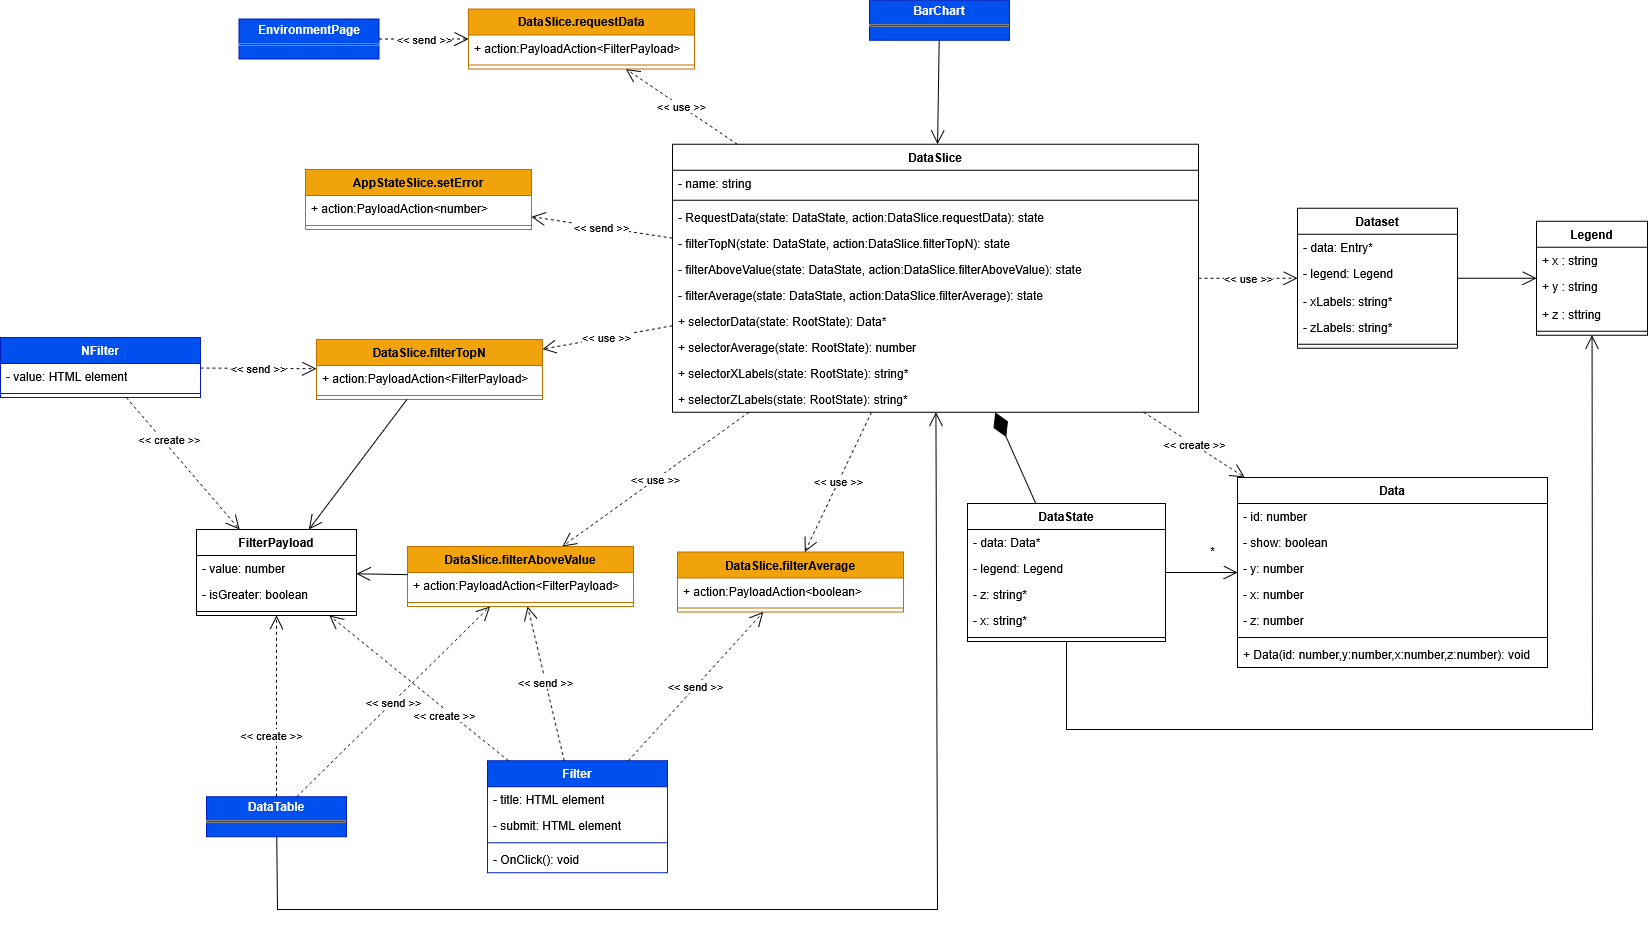
\includegraphics[scale=0.3]{template/images/uml_front/logic/dataslice.png}
    \caption{DataSlice}
\end{figure}
\textbf{Descrizione del diagramma:}\\
Questo diagramma include tutti i componenti utili per recuperare e filtrare i dati provenienti dal server.
\begin{itemize}
    \item \textbf{DataSlice:}
    \begin{itemize}
        \item \textbf{Dipendenze:}
        \begin{itemize}
            \item DataInitialState (composizione): gestisce la creazione e la distruzione dell'istanza di DataInitialState, che non è condivisa con altri componenti;
            \item RawData (dipendenza semplice <<use>>): recupera un singolo dato dal server di tipo RawData che verrà usato e convertito in Data;
            \item Data (dipendenza semplice <<create>>): responsabile della creazione dei singoli oggetti Data che verranno inseriti nella lista di dati di DataInitialState;
            \item DataSlice.requestData (dipendenza semplice <<use>>): cattura un'istanza di DataSlice.requestData e il reducer manda una richiesta al server per prendere i dati del dataset selezionato utilizzando il payload.
            \item DataSlice.filterTopN (dipendenza semplice <<use>>): cattura un'istanza di DataSlice.filterTopN e il reducer applica un filtro sui primi o gli ultimi N valori, basandosi sui parametri di FilterPayload.
            \item DataSlice.filterAverage (dipendenza semplice <<use>>): cattura un’istanza di DataSlice.filterAverage e il reducer applica un filtro sui valori maggiori o minori rispetto alla media globale, basandosi sui parametri di FilterPayload.
            \item DataSlice.filterAboveValue (dipendenza semplice <<use>>): cattura un’istanza di DataSlice.filterAboveValue e il reducer applica un filtro sui valori maggiori o minori rispetto ad un valore deciso dall'utente, basandosi sui parametri di FilterPayload.
            \item AppStateSlice.setError (dipendenza semplice <<send>>): crea ed emette un’istanza dell’azione AppStateSlice.setError.
        \end{itemize} 
        \item \textbf{Interazioni:}
        \begin{itemize}
            \item DataInitialState: viene modificato in base alle actions catturate dal reducer della slice.
        \end{itemize} 
        \item \textbf{Action catturate:}
        \begin{itemize}
            \item DataSlice.filterTopN
            \item DataSlice.filterAverage
            \item DataSlice.filterAboveValue
        \end{itemize} 
        \item \textbf{Action emesse:}
        \begin{itemize}
            \item AppStateSlice.setError
        \end{itemize} 
    \end{itemize}

    \item \textbf{DataInitialState:}
    \begin{itemize}
        \item \textbf{Dipendenze:}
        \begin{itemize}
            \item Data (associazione): contiene la lista dei dati del dataset.
        \end{itemize} 
    \end{itemize}

    \item \textbf{NFilter:}
    \begin{itemize}
        \item \textbf{Dipendenze:}
        \begin{itemize}
            \item DataSlice.filterTopN (dipendenza semplice <<send>>): crea ed emette un’istanza dell’azione DataSlice.filterTopN.
            \item FilterPayload (dipendenza semplice <<create>>): responsabile della creazione dei payload di tipo FilterPayload che verranno poi utilizzati per applicare un filtro nel modo corretto.
        \end{itemize} 
        \item \textbf{Action emesse:}
        \begin{itemize}
            \item DataSlice.filterTopN
        \end{itemize} 
    \end{itemize}

    \item \textbf{Filter:}
    \begin{itemize}
        \item \textbf{Dipendenze:}
        \begin{itemize}
            \item DataSlice.filterAverage (dipendenza semplice <<send>>): crea ed emette un’istanza dell’azione DataSlice.filterAverage.
            \item DataSlice.filterAboveValue (dipendenza semplice <<send>>): crea ed emette un’istanza dell’azione DataSlice.filterAboveValue.
            \item FilterPayload (dipendenza semplice <<create>>): responsabile della creazione dei payload di tipo FilterPayload che verranno poi utilizzati per applicare un filtro nel modo corretto.
        \end{itemize} 
        \item \textbf{Action emesse:}
        \begin{itemize}
            \item DataSlice.filterAverage;
            \item DataSlice.filterAboveValue.
        \end{itemize} 
    \end{itemize}

    \item \textbf{DataTable:}
    \begin{itemize}
        \item \textbf{Dipendenze:}
        \begin{itemize}
            \item DataSlice (associazione): contiene implicitamente un'istanza di DataSlice;
            \item DataSlice.filterAboveValue (dipendenza semplice <<send>>): crea ed emette un’istanza dell’azione DataSlice.DataSlice.
            \item FilterPayload (dipendenza semplice <<create>>): responsabile della creazione dei payload di tipo FilterPayload che verranno poi utilizzati per applicare un filtro nel modo corretto.
        \end{itemize} 
        \item \textbf{Interazioni:}
        \begin{itemize}
            \item DataSlice: vengono utilizzati i metodi selectorData,selectorXLabels e selectorZLabel per reperire la lista dei dati e delle etichette.
        \end{itemize} 
        \item \textbf{Action emesse:}
        \begin{itemize}
            \item DataSlice.filterAboveValue.
        \end{itemize} 
    \end{itemize}

    \item \textbf{BarChart:}
    \begin{itemize}
        \item \textbf{Dipendenze:}
        \begin{itemize}
            \item DataSlice (associazione): contiene implicitamente un'istanza di DataSlice;
        \end{itemize} 
        \item \textbf{Interazioni:}
        \begin{itemize}
            \item DataSlice: vengono utilizzati i metodi selectorData,selectorXLabels e selectorZLabel per reperire la lista dei dati e delle etichette.
        \end{itemize} 
    \end{itemize}

    \item \textbf{EnviroinmentPage:}
    \begin{itemize}
        \item \textbf{Dipendenze:}
        \begin{itemize}
            \item DataSlice.requestData (dipendenza semplice <<send>>): crea ed emette un’istanza dell’azione DataSlice.requestData .
        \end{itemize} 
        \item \textbf{Action emesse:}
        \begin{itemize}
            \item DataSlice.requestData ;
        \end{itemize} 
    \end{itemize}
\end{itemize}

\pagebreak

\paragraph{DataSourceSlice}
\begin{figure}[h!] \centering
    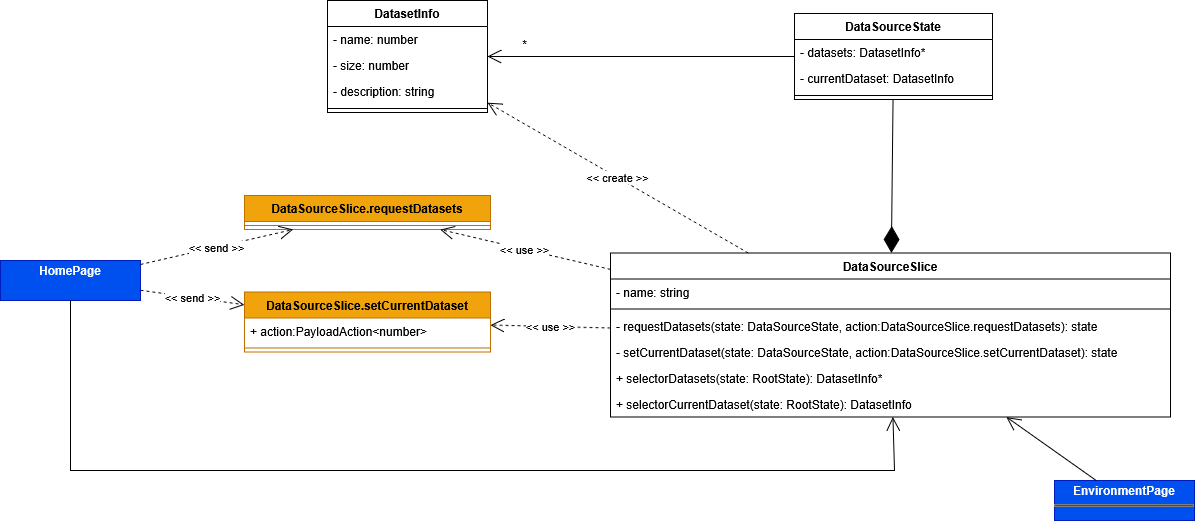
\includegraphics[scale=0.35]{template/images/uml_front/logic/datasourceslice.png}
    \caption{DataSourceSlice}
\end{figure}
\textbf{Descrizione del diagramma:}\\
Questo diagramma illustra i componenti per recuperare le informazioni chiave dai dataset proposti.
\begin{itemize}
    \item \textbf{DataSourceSlice:}
    \begin{itemize}
        \item \textbf{Dipendenze:}
        \begin{itemize}
            \item DataSourceInitialState (composizione): gestisce la creazione e la distruzione dell'istanza di DataSourceInitialState, che non è condivisa con altri componenti;;
            \item DatasetInfo (dipendenza semplice <<create>>):  responsabile della creazione dei singoli oggetti DatasetInfo che verranno inseriti nella lista di dataset di DataSourceInitialState;
            \item DataSourceSlice.requestData (dipendenza semplice <<use>>): cattura un'istanza di DataSourceSlice.requestData e il reducer manda una richiesta al server per prendere la lista dei dataset e le loro principali informazioni.
            \item DataSourceSlice.setCurrentDataset (dipendenza semplice <<use>>): cattura un'istanza di DataSourceSlice.setCurrentDataset e il reducer ne utilizza il payload per aggiornare il dataset selezionato dall'utente.
        \end{itemize} 
        \item \textbf{Interazioni:}
        \begin{itemize}
            \item DataSourceInitialState: viene modificato in base alle actions catturate dal reducer della slice.
        \end{itemize} 
        \item \textbf{Action catturate:}
        \begin{itemize}
            \item DataSourceSlice.setCurrentDataset
            \item DataSourceSlice.setCurrentDataset
        \end{itemize} 
    \end{itemize}

    
    \item \textbf{DataSourceInitialState:}
    \begin{itemize}
        \item \textbf{Dipendenze:}
        \begin{itemize}
            \item DatasetInfo (associazione): contiene la lista dei dataset proposti, con le loro informazioni, e quello corrente.
        \end{itemize} 
    \end{itemize}

    \item \textbf{SelectionPage:}
    \begin{itemize}
        \item \textbf{Dipendenze:}
        \begin{itemize}
            \item DataSource (associazione): contiene implicitamente un'istanza di DataSourceSlice;
            \item DataLabelSlice.requestData (dipendenza semplice <<send>>): crea ed emette un’istanza dell’azione DataLabelSlice.requestData.
            \item DataLabelSlice.setCurrentDataset (dipendenza semplice <<send>>): crea ed emette un’istanza dell’azione DataLabelSlice.setCurrentDataset.
        \end{itemize} 
        \item \textbf{Interazioni:}
        \begin{itemize}
            \item DataSource (associazione): viene utilizzato il metodo selectorDatasets per reperire la lista dei dati.
        \end{itemize} 
        \item \textbf{Action emesse:}
        \begin{itemize}
            \item DataLabelSlice.requestData
            \item DataLabelSlice.setCurrentDataset
        \end{itemize} 
    \end{itemize}

    \item \textbf{EnviroinmentPage:}
    \begin{itemize}
        \item \textbf{Dipendenze:}
        \begin{itemize}
            \item DataSource (associazione): contiene implicitamente un'istanza di DataSourceSlice;
        \end{itemize} 
        \item \textbf{Interazioni:}
        \begin{itemize}
            \item DataSource (associazione): viene utilizzato il metodo selectorCurrentDataset per reperire il dataset selezionato dall'utente e le sue informazioni.
        \end{itemize}  
    \end{itemize}
\end{itemize}

\paragraph{AppStateSlice}
\begin{figure}[h!] \centering
    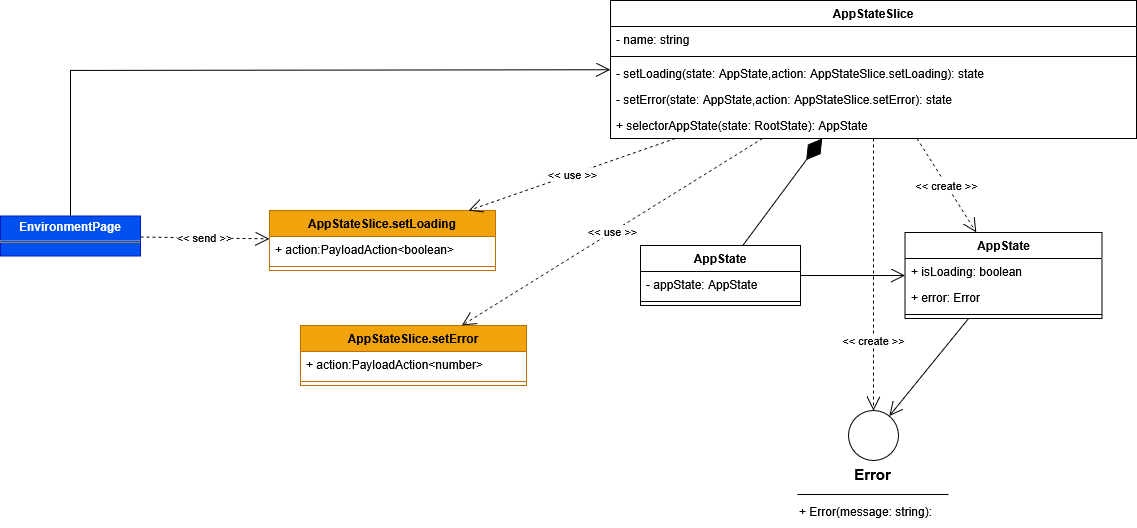
\includegraphics[scale=0.4]{template/images/uml_front/logic/appstateslice.png}
    \caption{AppStateSlice}
\end{figure}
\textbf{Descrizione del diagramma:}\\
Questo diagramma mostra i componenti per la gestione dello stato dell'applicazione.
\begin{itemize}
    \item \textbf{AppStateSlice:}
    \begin{itemize}
        \item \textbf{Dipendenze:}
        \begin{itemize}
            \item AppInitialState (composizione): gestisce la creazione e la distruzione dell'istanza di AppInitialState, che non è condivisa con altri componenti;
            \item AppState (dipendenza semplice <<create>>): responsabile della costruzione dell' oggetto AppState inserire all’interno dell AppInitialState;
            \item AppStateSlice.setLoading (dipendenza semplice <<use>>): cattura un’istanza di AppStateSlice.setLoading e il reducer aggiorna lo stato di caricamento dell'applicazione utilizzando il payload;
            \item AppStateSlice.setError (dipendenza semplice <<use>>): cattura un’istanza di AppStateSlice.setError e il reducer aggiorna lo stato di errore dell'applicazione ne utilizza il payload;
        \end{itemize} 
        \item \textbf{Interazioni:}
        \begin{itemize}
            \item DataSourceInitialState: viene modificato in base alle actions catturate dal reducer della slice.
        \end{itemize} 
        \item \textbf{Action catturate:}
        \begin{itemize}
            \item AppStateSlice.setLoading;
            \item AppStateSlice.setError.
        \end{itemize} 
    \end{itemize}

    
    \item \textbf{AppInitialState:}
    \begin{itemize}
        \item \textbf{Dipendenze:}
        \begin{itemize}
            \item AppState (associazione): contiene la l'oggetto che rappresenta lo stato dell'applicazione.
        \end{itemize} 
    \end{itemize}

    \item \textbf{EnviroinmentPage:}
    \begin{itemize}
        \item \textbf{Dipendenze:}
        \begin{itemize}
            \item AppStateSlice (associazione): contiene implicitamente un'istanza di AppStateSlice;
            \item AppStateSlice.setLoading (dipendenza semplice <<send>>):  crea ed emette un’istanza dell’azione AppStateSlice.setLoading;
        \end{itemize} 
        \item \textbf{Interazioni:}
        \begin{itemize}
            \item AppStateSlice (associazione): viene utilizzato il metodo selectorAppState per reperire lo stato dell'applicazione.
        \end{itemize}  
    \end{itemize}
\end{itemize}


\subparagraph{Error}
\begin{center}
    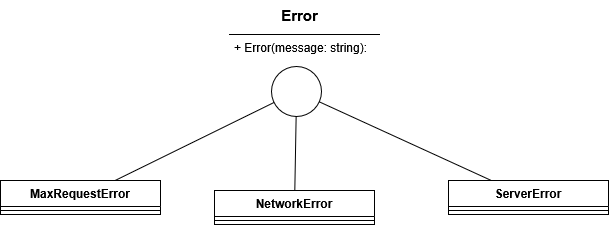
\includegraphics[scale=0.45]{template/images/uml_front/logic/error.png}
    % \caption{Error}
    \captionof{figure}{Error}
\end{center}
\textbf{Descrizione del diagramma:}\\
Questo diagramma mostra tutte le classi di errore.
\begin{itemize}
    \item \textbf{MaxRequestError:}
    \begin{itemize}
        \item \textbf{Dipendenze:}
        \begin{itemize}
            \item Error (implementazione): implementa una classe Error personalizzata, derivata da una superclasse Error esistente,
             che include un messaggio specifico per gli errori dovuti al superamento del limite di richieste.
        \end{itemize} 
    \end{itemize}

    \item \textbf{NetworkError:}
    \begin{itemize}
        \item \textbf{Dipendenze:}
        \begin{itemize}
            \item Error (implementazione): implementa una classe Error personalizzata, derivata da una superclasse Error esistente,
            che include un messaggio specifico per gli errori di rete non specifici.
        \end{itemize} 
    \end{itemize}

    \item \textbf{ServerError:}
    \begin{itemize}
        \item \textbf{Dipendenze:}
        \begin{itemize}
            \item Error (implementazione): implementa una classe Error personalizzata, derivata da una superclasse Error esistente,
            che include un messaggio specifico per gli errori di connessione non riuscita al server.
        \end{itemize} 
    \end{itemize}
\end{itemize}

\pagebreak

\paragraph{FilterOptionSlice}
\begin{figure}[h!] \centering
    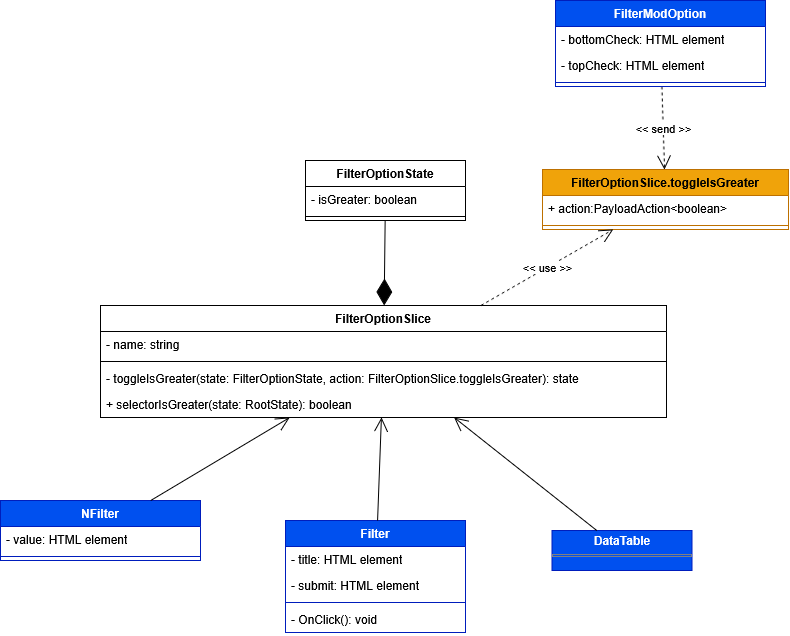
\includegraphics[scale=0.35]{template/images/uml_front/logic/filteroptionslice.png}
    \caption{FilterOptionSlice}
\end{figure}
\textbf{Descrizione del diagramma:}\\
Questo diagramma mostra i componenti per aggiornare e condividere le opzioni di filtraggio.
\begin{itemize}
    \item \textbf{FilterOptionSlice:}
    \begin{itemize}
        \item \textbf{Dipendenze:}
        \begin{itemize}
            \item FilterOptionInitialState (composizione): gestisce la creazione e la distruzione dell'istanza di FilterOptionInitialState, che non è condivisa con altri componenti;
            \item FilterOption (dipendenza semplice <<create>>): responsabile della costruzione dell'oggetto FilterOption da inserire all’interno della lista di dati di DataInitialState;
            \item FilterOption.toggleAveragePlane (dipendenza semplice <<use>>): cattura un’istanza di FilterOption.toggleAveragePlane e il reducer per impostare la visibilità del piano medio utilizzando il payload;
            \item FilterOption.toggleIsGreater (dipendenza semplice <<use>>): cattura un’istanza di FilterOption.toggleIsGreater e il reducer impostare il tipo di filtraggio da effettuare utilizzando il payload.
        \end{itemize} 
        \item \textbf{Interazioni:}
        \begin{itemize}
            \item FilterOptionInitialState: viene modificato in base alle actions catturate dal reducer della slice.
        \end{itemize} 
        \item \textbf{Action catturate:}
        \begin{itemize}
            \item FilterOption.toggleAveragePlane
            \item FilterOption.toggleIsGreater
        \end{itemize} 
    \end{itemize}

    \item \textbf{FilterOptionInitialState:}
    \begin{itemize}
        \item \textbf{Dipendenze:}
        \begin{itemize}
            \item FilterOption (associazione): contiene le opzioni di filtraggio correnti.
        \end{itemize} 
    \end{itemize}

    \item \textbf{NFilter:}
    \begin{itemize}
        \item \textbf{Dipendenze:}
        \begin{itemize}
            \item FilterOptionSlice (associazione): contiene implicitamente un'istanza di FilterOptionSlice;
        \end{itemize} 
        \item \textbf{Interazioni:}
        \begin{itemize}
            \item FilterOptionSlice: viene utilizzato il metodo selectorFilterOption per reperire le opzioni per il filtraggio.
        \end{itemize} 
    \end{itemize}

    \item \textbf{Filter:}
    \begin{itemize}
        \item \textbf{Dipendenze:}
        \begin{itemize}
            \item FilterOptionSlice (associazione): contiene implicitamente un'istanza di FilterOptionSlice;
        \end{itemize} 
        \item \textbf{Interazioni:}
        \begin{itemize}
            \item FilterOptionSlice: viene utilizzato il metodo selectorFilterOption per reperire le opzioni per il filtraggio.
        \end{itemize} 
    \end{itemize}

    \item \textbf{DataTable:}
    \begin{itemize}
        \item \textbf{Dipendenze:}
        \begin{itemize}
            \item FilterOptionSlice (associazione): contiene implicitamente un'istanza di FilterOptionSlice;
        \end{itemize} 
        \item \textbf{Interazioni:}
        \begin{itemize}
            \item FilterOptionSlice: viene utilizzato il metodo selectorFilterOption per reperire le opzioni per il filtraggio.
        \end{itemize} 
    \end{itemize}

    \item \textbf{AvgPlaneOption:}
    \begin{itemize}
        \item \textbf{Dipendenze:}
        \begin{itemize}
            \item FilterOption.toggleAveragePlane (associazione semplice <<send>>): crea ed emette un’istanza dell’azione FilterOption.toggleAveragePlane;
        \end{itemize} 
    \end{itemize}

    \item \textbf{FilterModOption:}
    \begin{itemize}
        \item \textbf{Dipendenze:}
        \begin{itemize}
            \item FilterOption.toggleIsGreater (associazione semplice <<send>>): crea ed emette un’istanza dell’azione FilterOption.toggleIsGreater;
        \end{itemize} 
    \end{itemize}
\end{itemize}

\paragraph{RaycastHitSlice}
\begin{figure}[h!] \centering
    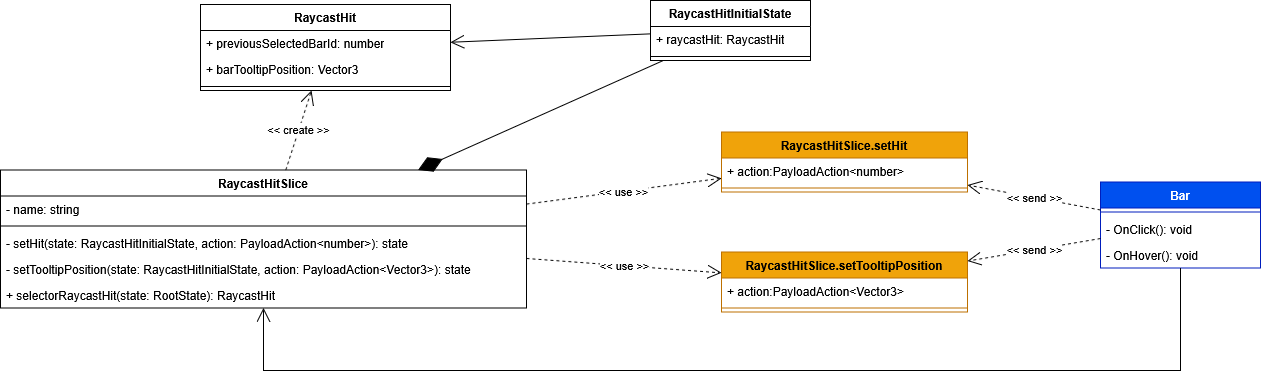
\includegraphics[scale=0.35]{template/images/uml_front/logic/raycasthitslice.png}
    \caption{RaycastHitSlice}
\end{figure}
\textbf{Descrizione del diagramma:}\\
Questo diagramma mostra i componenti per aggiornare e condividere le informazioni del raycast.
\begin{itemize}
    \item \textbf{RaycastHitSlice:}
    \begin{itemize}
        \item \textbf{Dipendenze:}
        \begin{itemize}
            \item RaycastHitInitialState (composizione): gestisce la creazione e la distruzione dell'istanza di RaycastHitInitialState, che non è condivisa con altri componenti;
            \item RaycastHit (dipendenza semplice <<create>>): responsabile della costruzione del RaycastHit da inserire all’interno dell RaycastHitInitialState;
            \item RaycastHitSlice.setHit (dipendenza semplice <<use>>): cattura un’istanza di RaycastHitSlice.setHit e il reducer memorizza la barra del grafico cliccata dall'utente utilizzando il payload;
            \item RaycastHitSlice.setTooltipPosition (dipendenza semplice <<use>>): cattura un’istanza di AppStateSlice.setError e il reducer aggiorna la posizione del tooltip utilizzando il payload;
        \end{itemize} 
        \item \textbf{Interazioni:}
        \begin{itemize}
            \item DataSourceInitialState: viene modificato in base alle actions catturate dal reducer della slice.
        \end{itemize} 
        \item \textbf{Action catturate:}
        \begin{itemize}
            \item RaycastHitSlice.setHit;
            \item RaycastHitSlice.setTooltipPosition.
        \end{itemize} 
    \end{itemize}

    
    \item \textbf{RaycastHitInitialState:}
    \begin{itemize}
        \item \textbf{Dipendenze:}
        \begin{itemize}
            \item RaycastHit (associazione): contiene la l'oggetto che rappresenta il punto di intersezione tra il mouse e una barra del grafico.
        \end{itemize} 
    \end{itemize}

    \item \textbf{Raycaster:}
    \begin{itemize}
        \item \textbf{Dipendenze:}
        \begin{itemize}
            \item RaycastHitSlice (associazione):  contiene implicitamente un'istanza di RaycastHitSlice;
            \item RaycastHitSlice.setHit (dipendenza semplice <<send>>):  crea ed emette un’istanza dell’azione RaycastHitSlice.setHit;
            \item RaycastHitSlice.setToolTipPosition (dipendenza semplice <<send>>):  crea ed emette un’istanza dell’azione RaycastHitSlice.setToolTipPosition;
        \end{itemize} 
        \item \textbf{Interazioni:}
        \begin{itemize}
            \item RaycastHitSlice: viene utilizzato i metodo selectorRaycastHit per reperire le informazioni del raycast.
        \end{itemize}  
    \end{itemize}
\end{itemize}

\paragraph{Redux store}
\begin{figure}[h!] \centering
    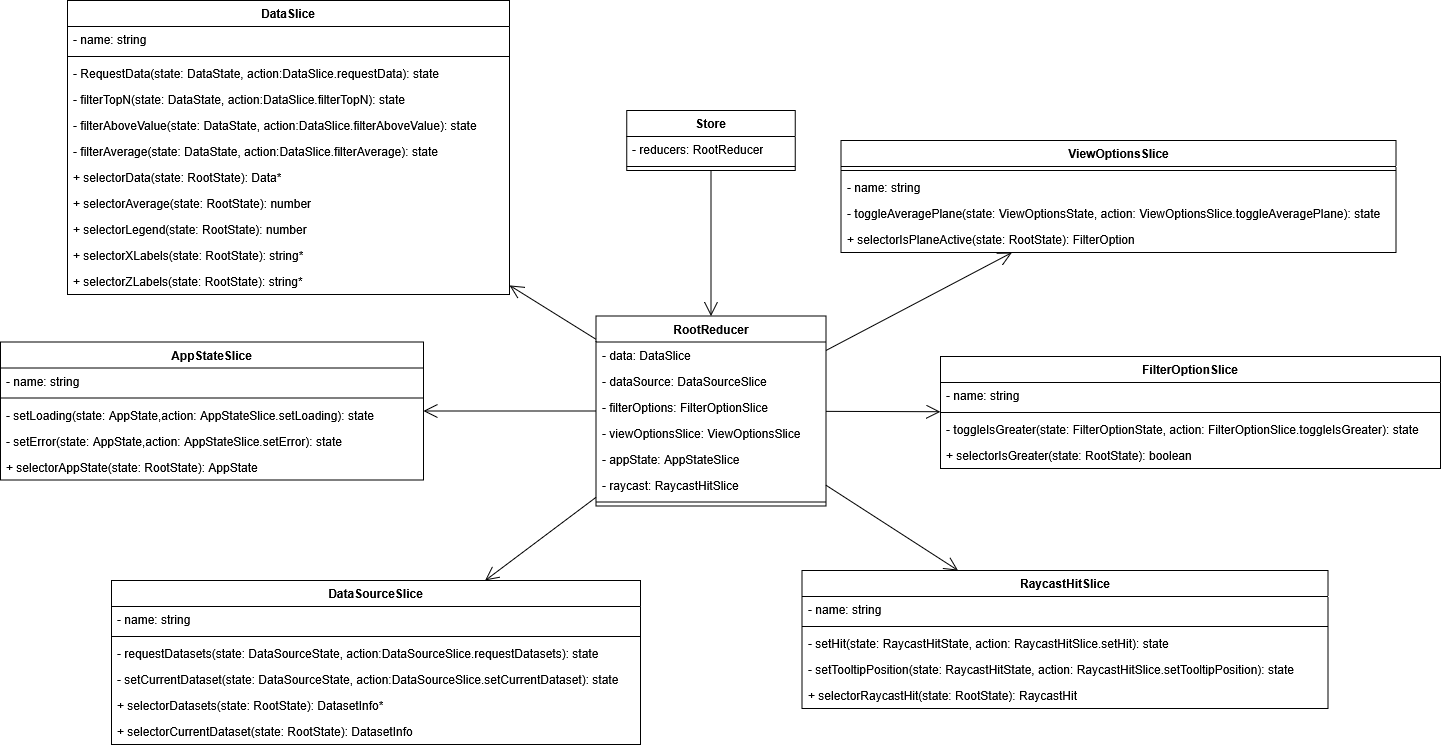
\includegraphics[scale=0.3]{template/images/uml_front/logic/store.png}
    \caption{Redux store}
\end{figure}
\textbf{Descrizione del diagramma:}\\
Questo diagramma mostra lo store e gli slice che compongono lo stato globale dell'applicazione.
\begin{itemize}
    \item \textbf{Store:}
    \begin{itemize}
        \item \textbf{Dipendenze:}
        \begin{itemize}
            \item RootReducer (associazione): possiede un attributo RootReducer che permette di combinare pi´u slice
            con cui lo store interagisce per modificare lo stato globale dell’applicazione;
        \end{itemize}  
    \end{itemize}

    \item \textbf{RootReducer:}
    \begin{itemize}
        \item \textbf{Dipendenze:}
        \begin{itemize}
            \item DataSlice (associazione): possiede un attributo DataSlice per offrire allo store l’accesso alla slice.
            \item DataSourceSlice (associazione): possiede un attributo DataSourceSlice per offrire allo store l’accesso alla slice.
            \item FilterOptionSlice (associazione): possiede un attributo FilterOptionSlice per offrire allo store l’accesso alla slice.
            \item AppStateSlice (associazione): possiede un attributo AppStateSlice per offrire allo store l’accesso alla slice.
            \item RaycastHitSlice (associazione): possiede un attributo RaycastHitSlice per offrire allo store l’accesso alla slice.
        \end{itemize}  
    \end{itemize}
\end{itemize}


Spostando l'attenzione sulla creazione dell'interfaccia utente e sulle dipendenze dei componenti React:

\paragraph{Pages}
\begin{figure}[h!] \centering
    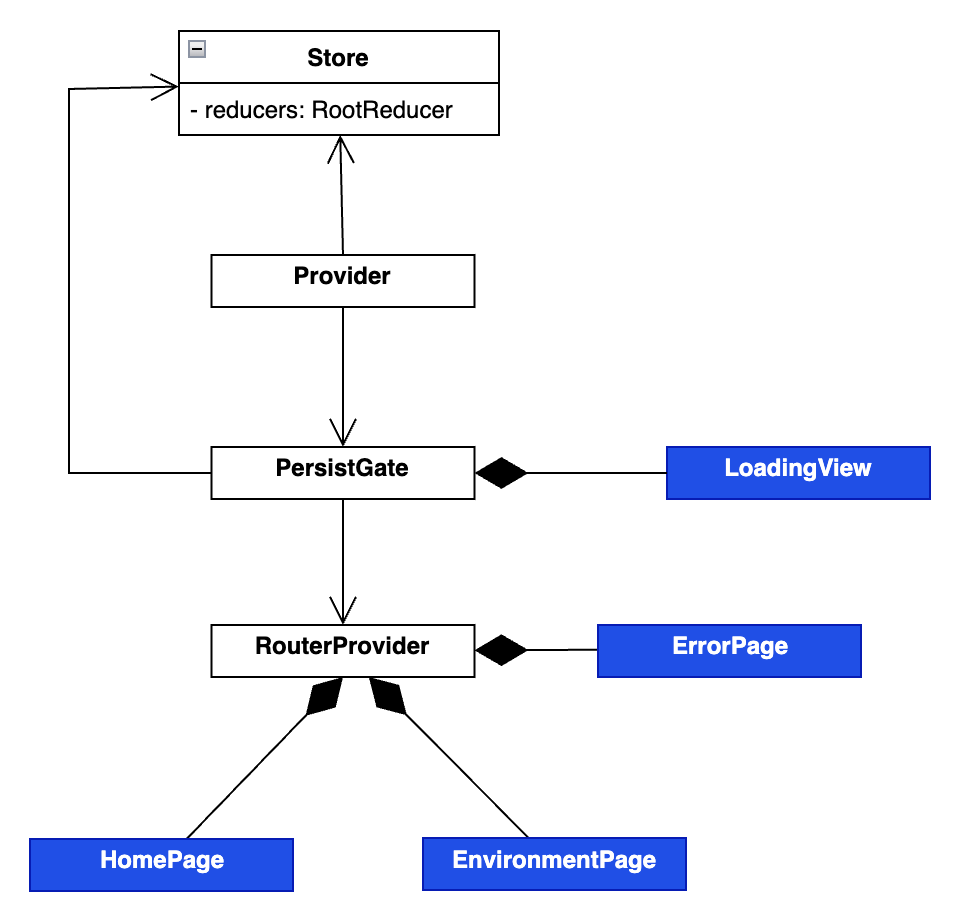
\includegraphics[scale=0.45]{template/images/uml_front/ui/pages.png}
    \caption{Pages}
\end{figure}
\textbf{Descrizione del diagramma:}
Questo diagramma mostra come sono organizzate le varie pagine dell'applicazione web.
\begin{itemize}
    \item \textbf{Provider:}
    \begin{itemize}
        \item \textbf{Dipendenze:}
        \begin{itemize}
            \item Store (associazione): utile al Provider di Redux per consentire l'accesso allo store (e quindi allo stato globale) a tutti i componenti nella gerarchia.
            \item RouterProvider (associazione): componente React che contiene le pagine dell'applicazione web con i loro relativi percorsi;
        \end{itemize} 
    \end{itemize}

    \item \textbf{SelectionPage:}
    \begin{itemize}
        \item \textbf{Dipendenze:}
        \begin{itemize}
            \item SelectionPage (composizione): componente React che rappresenta la pagina di selezione del dataset.
            \item EnviroinmentPage (composizione): componente React che rappresenta la pagina di visualizzazione del dataset nell'ambiente tridimensionale.
            \item RouterErrorPage (composizione): componente React che rappresenta la pagina di visualizzazione di eventuali errori generati dall'applicazione.
        \end{itemize} 
    \end{itemize}

    \item \textbf{SelectionPage:}
    \begin{itemize}
        \item \textbf{Dipendenze:}
        \begin{itemize}
            \item DatasetItem (composizione): componente React che rappresenta un singolo dataset con le sue informazioni principali.
        \end{itemize} 
    \end{itemize}
\end{itemize}

\paragraph{EnviroinmentPage}
\begin{figure}[h!] \centering
    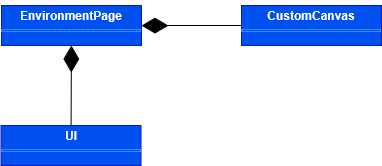
\includegraphics[scale=0.45]{template/images/uml_front/ui/envpage.png}
    \caption{EnviroinmentPage}
\end{figure}
\textbf{Descrizione del diagramma:}
Questo diagramma mostra l'organizzazione della pagina dedicata all'ambiente tridimensionale.
\begin{itemize}
    \item \textbf{EnviroinmentPage:}
    \begin{itemize}
        \item \textbf{Dipendenze:}
        \begin{itemize}
            \item UI (composizione): componente React che racchiude tutta la UI dell'applicazione web.
            \item CustomCanvas (composizione): componente React che racchiude l'ambiente tridimensionale.
        \end{itemize} 
    \end{itemize}
\end{itemize}

\paragraph{UI}
\begin{figure}[h!] \centering
    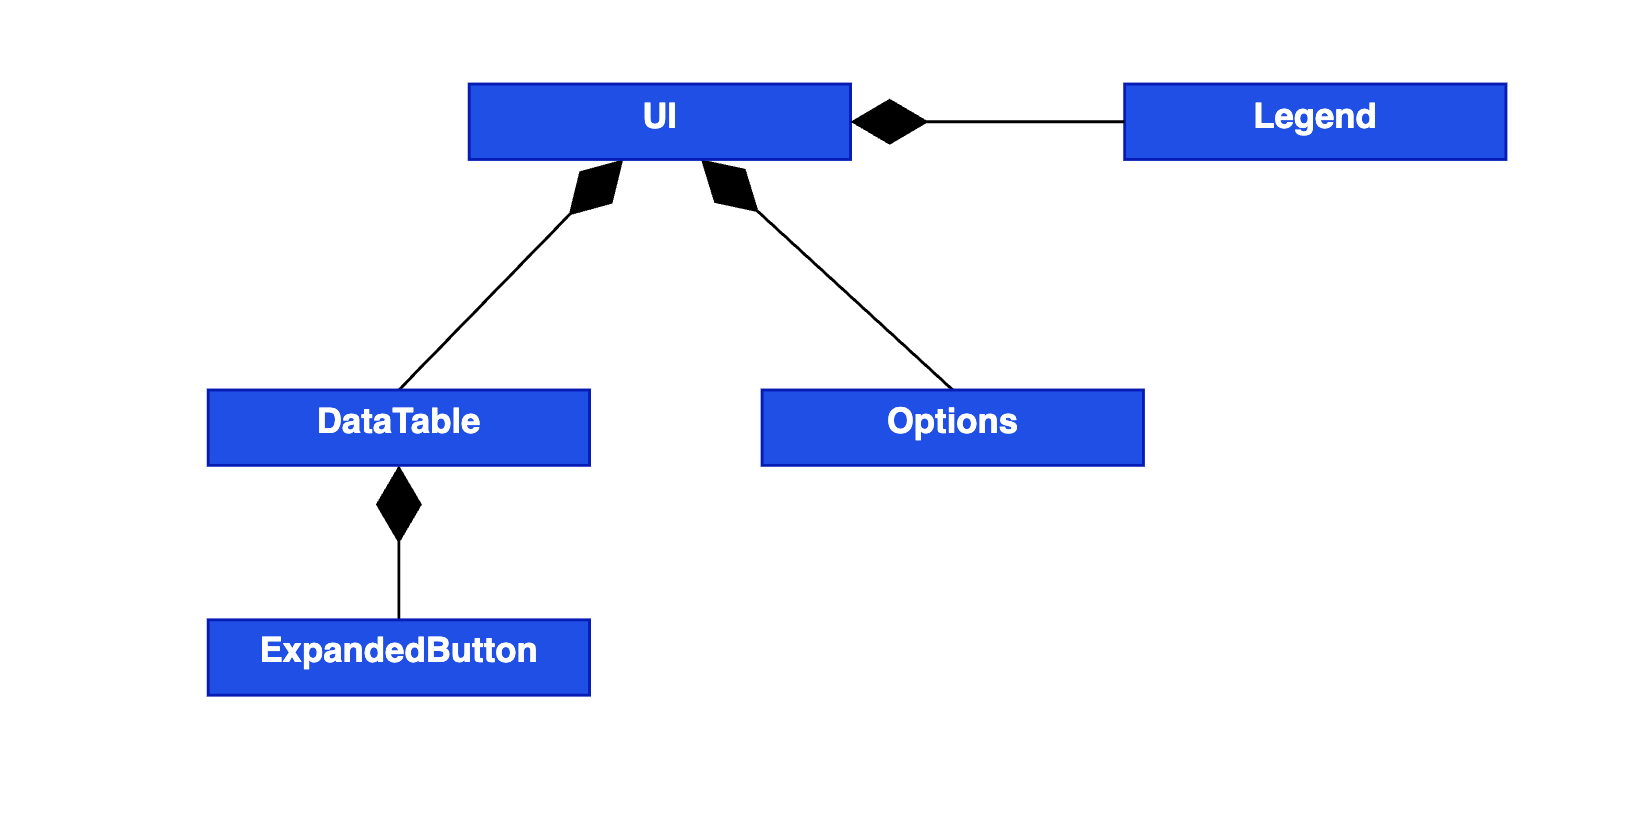
\includegraphics[scale=0.45]{template/images/uml_front/ui/ui.png}
    \caption{UI}
\end{figure}
\textbf{Descrizione del diagramma:}
Questo diagramma mostra come è composta la parte UI dell'applicazione.
\begin{itemize}
    \item \textbf{UI:}
    \begin{itemize}
        \item \textbf{Dipendenze:}
        \begin{itemize}
            \item Footer (composizione): componente React che rappresenta il footer dell'applicazione web.
            \item DataTable (composizione): componente React che rappresenta il dataset in forma tabellare.
            \item FilterOptions (composizione): componente React che rappresenta il form con le opzioni di filtraggio.
        \end{itemize} 
    \end{itemize}
\end{itemize}

\pagebreak

\paragraph{Filter options}
\begin{figure}[h!] \centering
    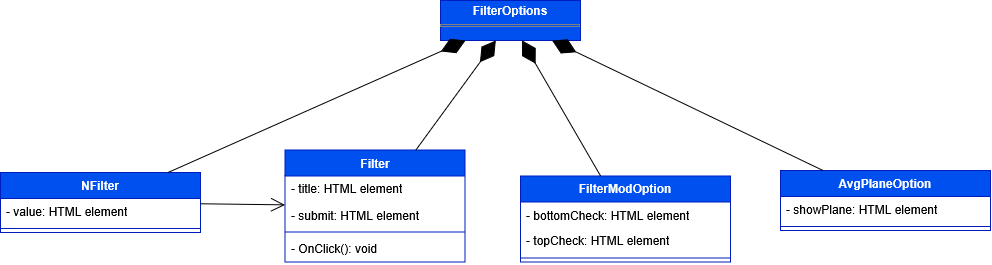
\includegraphics[scale=0.45]{template/images/uml_front/ui/filteroptions.png}
    \caption{Filter options}
\end{figure}
\textbf{Descrizione del diagramma:}
Questo diagramma mostra come sono raggruppati le opzioni di filtraggio.
\begin{itemize}
    \item \textbf{FilterOption:}
    \begin{itemize}
        \item \textbf{Dipendenze:}
        \begin{itemize}
            \item NFilter (composizione): componente React che rappresenta il filtro su i top o bottom N valori.
            \item Filter (composizione): componente React che rappresenta un filtro generico che di base può filtrare per valori maggiori o minori rispetto ad un altro.
            \item FilterModOption (composizione): componente React che rappresenta il form per decidere se il filtro avverrà per valori minori o maggiori.
            \item AvgPlaneOption (composizione): componente React che rappresenta il form per decidere se rendere visibile il piano del valor medio.
        \end{itemize} 
    \end{itemize}

    \item \textbf{NFilter:}
    \begin{itemize}
        \item \textbf{Dipendenze:}
        \begin{itemize}
            \item Filter (associazione): componente React che rappresenta un filtro generico che di base può filtrare per valori maggiori o minori rispetto ad un altro.
            in questo caso è stato utilizzato per estendere la sua funzionalità aggiungendo un campo per la decisione di un valore N.
        \end{itemize} 
    \end{itemize}
\end{itemize}

\paragraph{Custom canvas}
\begin{figure}[h!] \centering
    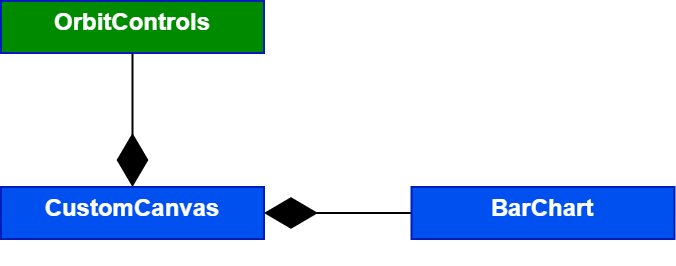
\includegraphics[scale=0.45]{template/images/uml_front/ui/customcanvas.png}
    \caption{Custom canvas}
\end{figure}
\textbf{Descrizione del diagramma:}
Questo diagramma mostra come è composto l'ambiente tridimensionale.
\begin{itemize}
    \item \textbf{CustomCanvas:}
    \begin{itemize}
        \item \textbf{Dipendenze:}
        \begin{itemize}
            \item OrbitControls (composizione): componente React three fiber utile per implementare i movimenti della vista attraverso il mouse.
            \item BarChart (composizione): componente React che rappresenta l'intero grafico tridimensionale.
        \end{itemize} 
    \end{itemize}
\end{itemize}

\pagebreak

\paragraph{Bar chart}
\begin{figure}[h!] \centering
    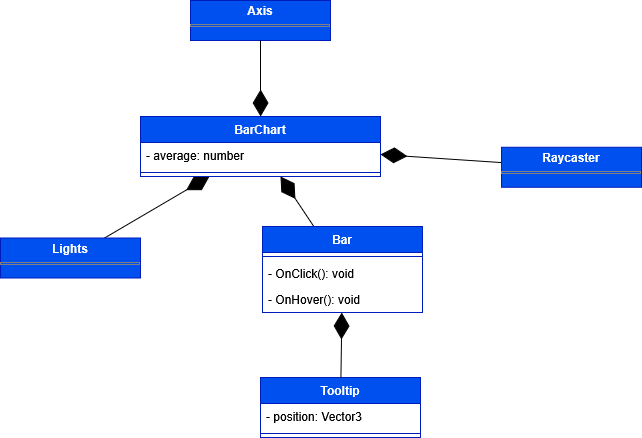
\includegraphics[scale=0.45]{template/images/uml_front/ui/barchart.png}
    \caption{Bar chart}
\end{figure}
\textbf{Descrizione del diagramma:}
Questo diagramma mostra quali sono le componenti del grafico tridimensionale
\begin{itemize}
    \item \textbf{BarChart:}
    \begin{itemize}
        \item \textbf{Dipendenze:}
        \begin{itemize}
            \item Axis (composizione): componente React che racchiude gli assi X, Y e Z del grafico tridimensionale.
            \item Lights (composizione): componente React che racchiude e gestisce luci dell'ambiente tridimensionale.
            \item Raycaster (composizione): componente React che rappresenta l'intersezione tra il punto di intersezione tra il mouse e una barra del grafico..
            \item Bar (composizione): componente React che rappresenta le barre del grafico tridimensionale.
        \end{itemize} 
    \end{itemize}

    \item \textbf{Bart:}
    \begin{itemize}
        \item \textbf{Dipendenze:}
        \begin{itemize}
            \item Tooltip (composizione): componente React che rappresenta un piccolo riquadro informativo riguardo dalla barra del grafico selezionata.
        \end{itemize} 
    \end{itemize}
\end{itemize}

\paragraph{Axis}
\begin{figure}[h!] \centering
    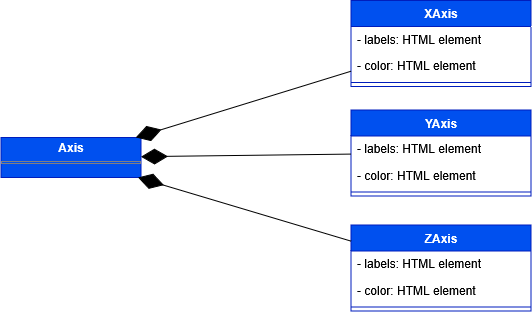
\includegraphics[scale=0.45]{template/images/uml_front/ui/axis.png}
    \caption{Axis}
\end{figure}
\textbf{Descrizione del diagramma:}
Questo diagramma mostra i componenti che formano i 3 assi del grafico tridimensionale.
\begin{itemize}
    \item \textbf{Axis:}
    \begin{itemize}
        \item \textbf{Dipendenze:}
        \begin{itemize}
            \item XAxis (composizione): componente React che rappresenta l'asse X del grafico tridimensionale con le relative etichette.
            \item YAxis (composizione): componente React che rappresenta l'asse Y del grafico tridimensionale con le relative etichette.
            \item ZAxis (composizione): componente React che rappresenta l'asse Z del grafico tridimensionale con le relative etichette.
        \end{itemize} 
    \end{itemize}
\end{itemize}




